\documentclass[12pt, oneside, openany]{book}
\usepackage[utf8]{inputenc}
\usepackage[T1]{fontenc}
\usepackage[spanish]{babel}
\usepackage{enumitem}
\usepackage{amsmath,amssymb}
\usepackage[letterpaper,left=2.0cm,right=2.0cm,top=2.5cm,bottom=2.5cm]{geometry}
\usepackage{graphicx}
\usepackage{siunitx}
\usepackage{float}
\usepackage{natbib}
\usepackage{setspace}
\onehalfspacing
\usepackage{textgreek}
\usepackage{caption}
\usepackage{csquotes}
\usepackage{booktabs}
\usepackage{listings}
\usepackage{xcolor}
\usepackage{subcaption}
\usepackage{matlab-prettifier}
\usepackage{hyperref}

\hypersetup{
    colorlinks=true,
    linkcolor=blue,
    urlcolor=blue,
    citecolor=blue
}

% --- Portada ---
\title{
    {\Large \textbf{UNIVERSIDAD TÉCNICA FEDERICO SANTA MARÍA}}\\[1mm]
    {\large DEPARTAMENTO DE ELECTRÓNICA}\\[1mm]
    % La imagen se mantiene, asumiendo que estará disponible durante la compilación.
    \includegraphics[width=4.5cm]{Logo_UTFSM.png}\\[2mm]
    {\Large \textbf{Tarea 1 | Agentes de Búsqueda y Aprendizaje por Refuerzo}}\\[2mm]
    {\Large TEL351 - Seminario de Telemática I - 2025-2}\\[1mm]
    {\large Fecha de entrega: Lunes, 22 de Septiembre de 2025}\\[0.5mm]
    {\normalsize PROFESOR:}\\[0.5mm]
    {\normalsize Mauricio Araya}\\[0.5mm]
    {\normalsize ALUMNOS:}\\[0.5mm]
    {\normalsize 
    Javier Cáceres León - 202030032-1}\\[0.5mm]
    {\normalsize Cristóbal Moraga Guerrero - 202130008-2}\\[0.5mm]
    {\normalsize Camilo Troncoso Hormazabal - 202130004-K}\\[0.5mm]
}

% Definición de colores para el código
\definecolor{codegreen}{rgb}{0,0.6,0}
\definecolor{codegray}{rgb}{0.5,0.5,0.5}
\definecolor{codepurple}{rgb}{0.58,0,0.82}
\definecolor{backcolour}{rgb}{0.95,0.95,0.92}

% Estilo mejorado para los listados de código
\lstdefinestyle{mystyle}{
    backgroundcolor=\color{backcolour},   
    commentstyle=\color{codegreen}\itshape,
    keywordstyle=\color{magenta}\bfseries,
    numberstyle=\tiny\color{codegray},
    stringstyle=\color{codepurple},
    basicstyle=\footnotesize\ttfamily,
    breakatwhitespace=false,         
    breaklines=true,                 
    captionpos=b,                    
    keepspaces=true,                 
    numbers=left,                    
    numbersep=5pt,                  
    showspaces=false,                
    showstringspaces=false,
    showtabs=false,                  
    tabsize=2,
    frame=single,
    framerule=0.5pt,
    rulecolor=\color{black}
}
\lstset{style=mystyle}

\author{}
\date{}

\begin{document}
\maketitle
\tableofcontents
\newpage

\section{Introducción}
El presente informe técnico detalla el análisis, implementación y evaluación comparativa de diversas familias de agentes inteligentes en el contexto del videojuego \textit{Pokémon Rojo}. El objetivo principal de los agentes es resolver una tarea específica y fundamental: la selección del Pokémon inicial en el menor tiempo o número de pasos posible. Este problema, aunque aparentemente simple, encapsula desafíos clave en el campo de la inteligencia artificial, como la navegación en entornos parcialmente observables, la interacción con menús y la toma de decisiones secuencial.

Para abordar este desafío, se exploran y comparan tres familias de estrategias algorítmicas, abarcando desde búsquedas clásicas hasta métodos avanzados de aprendizaje por refuerzo (RL):
\begin{itemize}
    \item \textbf{Algoritmos de Búsqueda Clásicos}: Métodos informados y no informados (como A*, BFS y Hill Climbing) que planifican una ruta basándose en un modelo explícito del entorno.
    \item \textbf{Aprendizaje por Refuerzo Simple (Epsilon-Greedy)}: Un enfoque que equilibra la exploración y la explotación para aprender una política de acción a través de la experiencia, sin un modelo complejo.
    \item \textbf{Aprendizaje por Refuerzo Profundo (PPO)}: Un algoritmo de última generación que utiliza redes neuronales profundas para aprender una política óptima directamente desde las observaciones de píxeles, sin conocimiento previo del dominio.
\end{itemize}

El informe se estructura en torno a siete preguntas fundamentales que guían el análisis, desde la selección y comprensión del entorno de simulación hasta la implementación y comparación cuantitativa de los algoritmos. Se presentarán tablas, gráficos y conclusiones derivadas del análisis de datos experimentales recopilados de 143 ejecuciones, con el fin de ofrecer una evaluación rigurosa y autocontenida del rendimiento de cada estrategia. El énfasis no recae únicamente en el éxito de una estrategia sobre otra, sino en el proceso analítico y la comprensión profunda de sus fortalezas, debilidades y compromisos inherentes en este dominio particular.

\section{El Mundo de Pokémon Rojo: Un Contexto para la IA}
\label{sec:contexto_pokemon}

Para comprender la magnitud del desafío que enfrenta un agente de inteligencia artificial en este proyecto, es fundamental entender el universo del juego en el que opera: \textit{Pokémon Rojo}. Lanzado en 1996, este título no fue diseñado con la IA moderna en mente, lo que presenta un conjunto de retos únicos que no se encuentran en entornos de aprendizaje por refuerzo tradicionales como los de OpenAI Gym.

\subsection{Mecánicas Fundamentales del Juego}
\textit{Pokémon Rojo} es un juego de rol (RPG) donde el jugador asume el papel de un joven entrenador Pokémon. El objetivo principal es viajar por la región de Kanto para convertirse en el campeón de la Liga Pokémon. Esto implica:
\begin{itemize}
    \item \textbf{Exploración:} Navegar un mundo 2D basado en baldosas, que incluye ciudades, rutas, cuevas y edificios. El movimiento está restringido a una cuadrícula, y el entorno contiene tanto caminos abiertos como obstáculos (árboles, agua, paredes).
    \item \textbf{Captura de Pokémon:} Encontrar Pokémon salvajes en la hierba alta o en cuevas y capturarlos usando objetos llamados Poké Balls.
    \item \textbf{Batallas por Turnos:} Luchar contra otros entrenadores o Pokémon salvajes en un sistema de combate por turnos. Cada Pokémon tiene estadísticas, tipos y hasta cuatro movimientos, creando un sistema de fortalezas y debilidades similar al "piedra, papel o tijera", pero con 15 tipos diferentes.
    \item \textbf{Progresión y Objetivos:} La progresión es semi-lineal. Se deben completar ciertos objetivos (como derrotar a un líder de gimnasio) para desbloquear nuevas áreas o habilidades (como la capacidad de cortar árboles que bloquean un camino).
\end{itemize}

\subsection{El Objetivo Inicial: La Primera Decisión Crítica}
El alcance de este informe se centra en la primera tarea crucial del juego: \textbf{elegir el Pokémon inicial}. Al comienzo de la aventura, el jugador se encuentra en el laboratorio del Profesor Oak y debe seleccionar uno de tres Pokémon: Bulbasaur, Charmander o Squirtle.

\begin{figure}[H]
    \centering
    \includegraphics[width=1\textwidth]{3cf5c11a-703f-4a37-a774-85a4b9ed6d26-6.png}
    \caption{Visualización del mapa del juego y el agente navegando por el mapa.}
    \label{fig:poke_map}
\end{figure}

Aunque parece una tarea simple para un humano, para un agente de IA representa un problema de navegación y toma de decisiones con las siguientes características:
\begin{enumerate}
    \item \textbf{Navegación desde un Estado Inicial:} El agente comienza en su habitación y debe encontrar la salida de su casa.
    \item \textbf{Exploración del Pueblo:} Una vez fuera, debe navegar por Pueblo Paleta, un pequeño entorno con varios edificios y personajes no jugables (NPCs).
    \item \textbf{Activación de Eventos (Triggers):} El agente no puede simplemente entrar al laboratorio y elegir. Primero debe intentar salir del pueblo por el norte, lo que activa un evento donde el Profesor Oak lo detiene y lo guía a su laboratorio. Sin este paso, el objetivo es inalcanzable.
    \item \textbf{Interacción con Objetos:} Dentro del laboratorio, debe caminar hasta la mesa correcta y presionar un botón de acción frente a una de las tres Poké Balls para hacer su elección.
\end{enumerate}

Este primer objetivo encapsula los desafíos de navegación, secuenciación de eventos y interacción con el entorno que son fundamentales en todo el juego, sirviendo como un excelente microcosmos para evaluar la eficacia de diferentes estrategias de IA.

\section{Análisis del Entorno y Requisitos del Proyecto}
\label{sec:analisis_entorno}

\subsection{Complejidad del Entorno de Aprendizaje}
El entorno de \textit{Pokémon Rojo}, facilitado por el emulador \textbf{PyBoy}, es significativamente más complejo que los entornos de benchmark estándar. Su complejidad se puede desglosar en varios ejes:

\begin{itemize}
    \item \textbf{Espacio de Observación Gigantesco:} A diferencia de entornos que devuelven un vector de estado simple, el agente recibe la pantalla del juego como una matriz de píxeles (144x160 píxeles en escala de grises). Esto constituye un espacio de observación de alta dimensionalidad ($144 \times 160 = 23,040$ valores) que requiere un pre-procesamiento significativo o el uso de redes neuronales convolucionales (CNNs) para extraer características relevantes.
    \item \textbf{Espacio de Acciones Discreto pero Combinatorio:} El agente puede realizar acciones básicas como moverse (arriba, abajo, izquierda, derecha) o presionar botones (A, B, Start, Select). Aunque el número de acciones es pequeño (típicamente 8), las secuencias de estas acciones pueden tener efectos complejos y retardados. Por ejemplo, navegar un menú para usar un objeto requiere una secuencia precisa de múltiples pulsaciones de botones.
    \item \textbf{Recompensas Escasas y Retardadas (Sparse Rewards):} Este es uno de los mayores desafíos. En el objetivo de elegir el Pokémon inicial, el agente solo recibe una recompensa positiva significativa al final de una larga secuencia de acciones. Durante la mayor parte de la exploración, no hay una señal clara que le indique si está progresando. Esto hace que los algoritmos que dependen de retroalimentación constante (como Q-Learning simple) sean ineficaces sin una ingeniería de recompensas cuidadosa.
    \item \textbf{Parcialmente Observable (POMDP):} El agente solo ve la pantalla actual. No tiene acceso directo a la memoria completa del juego (por ejemplo, el estado de los eventos o la ubicación de los objetos fuera de la pantalla). Debe inferir el estado del mundo a partir de una secuencia de observaciones, lo que lo convierte en un Problema de Decisión de Markov Parcialmente Observable (POMDP).
    \item \textbf{Entorno No Determinista (Estocástico):} Aunque el emulador en sí es determinista, las interacciones con NPCs o Pokémon salvajes pueden introducir un comportamiento estocástico, alterando el flujo del juego de manera impredecible.
\end{itemize}

En resumen, el entorno es suficientemente complejo para un proyecto de esta envergadura, ya que combina desafíos de visión por computadora, planificación a largo plazo, exploración en un mundo con recompensas escasas y la necesidad de manejar una alta dimensionalidad tanto en el estado como en la secuencia de acciones.

\subsection{Instalación y Dependencias}
El proyecto se basa en un repositorio de código abierto con una comunidad activa. La instalación requiere una configuración precisa para asegurar la compatibilidad entre el emulador, las librerías de aprendizaje por refuerzo y el sistema operativo.

\subsubsection{Requisitos Previos}
\begin{itemize}
    \item \textbf{Python:} Se recomienda la versión 3.10 o superior.
    \item \textbf{ROM del Juego:} Es indispensable poseer una copia legal de la ROM de \textit{Pokémon Rojo}, renombrada a \texttt{PokemonRed.gb} y con un hash SHA-1 de \texttt{ea9bcae617fdf159b045185467ae58b2e4a48b9a}.
    \item \textbf{FFmpeg:} Una herramienta de software libre para manipular video y audio, necesaria para grabar las sesiones de entrenamiento.
    \item \textbf{Dependencias de C++:} En Windows, se requieren las "C++ Build Tools" de Visual Studio para compilar algunas de las dependencias de Python.
\end{itemize}

\subsubsection{Proceso de Instalación}
El proceso de instalación, detallado en los archivos \texttt{README.md} y \texttt{windows-setup-guide.md}, se puede resumir en los siguientes pasos:
\begin{enumerate}
    \item Clonar el repositorio desde GitHub.
    \item Crear un entorno virtual (por ejemplo, con \texttt{conda} o \texttt{venv}) para aislar las dependencias del proyecto.
    \item Instalar las librerías de Python especificadas en el archivo \texttt{requirements.txt} usando \texttt{pip}. Las dependencias clave incluyen:
    \begin{itemize}
        \item \texttt{pyboy}: El emulador de Game Boy.
        \item \texttt{gymnasium}: El toolkit para desarrollar y comparar algoritmos de RL.
        \item \texttt{stable-baselines3}: Un conjunto de implementaciones de algoritmos de RL de última generación.
        \item \texttt{torch}: La librería de computación tensorial utilizada por Stable Baselines3 para las redes neuronales.
        \item \texttt{pandas}, \texttt{matplotlib}, \texttt{seaborn}: Para el análisis y visualización de datos.
    \end{itemize}
    \item Colocar la ROM del juego en el directorio raíz del proyecto.
\end{enumerate}
Las pruebas realizadas durante este proyecto confirman que, siguiendo las guías proporcionadas, el entorno se ejecuta correctamente en un sistema Windows 11 con Python 3.12, demostrando la viabilidad de la configuración.

\section{Arquitectura del Agente y Estrategias Implementadas}
\label{sec:arquitectura_agentes}

Una de las fortalezas de este proyecto es la clara separación entre la lógica del agente y la simulación del entorno, lo que permite experimentar con diversas estrategias de IA sin modificar el núcleo del emulador.

\subsection{Separación Agente-Entorno}
El diseño sigue el paradigma estándar del aprendizaje por refuerzo, popularizado por OpenAI Gym:
\begin{itemize}
    \item \textbf{El Entorno (\texttt{RedGymEnv}):} El archivo \texttt{baselines/red\_gym\_env.py} define una clase, \texttt{RedGymEnv}, que hereda de \texttt{gym.Env}. Esta clase actúa como un wrapper alrededor del emulador PyBoy. Su responsabilidad es:
    \begin{enumerate}
        \item Iniciar y gestionar el estado del emulador.
        \item Definir el espacio de acciones y de observaciones.
        \item Implementar la función \texttt{step(action)}, que recibe una acción del agente, la ejecuta en el emulador, y devuelve la nueva observación, la recompensa, y si el episodio ha terminado.
        \item Implementar la función \texttt{reset()}, que reinicia el juego a un estado inicial.
    \end{enumerate}
    \item \textbf{El Agente:} El agente es una entidad separada que interactúa con el entorno a través de su API (\texttt{step} y \texttt{reset}). No tiene conocimiento de la implementación interna del entorno (es decir, no sabe que está usando PyBoy). Su única tarea es observar el estado y elegir una acción.
\end{itemize}

Esta separación es crucial, ya que permite que cualquier algoritmo, desde una simple búsqueda hasta una compleja red neuronal, pueda interactuar con el juego siempre que respete la interfaz definida por Gymnasium. Las pruebas de concepto realizadas en \texttt{comparison\_agents/} demuestran esto: se crearon múltiples agentes (\texttt{epsilon\_greedy\_agent.py}, \texttt{astar\_agent.py}, etc.) que operan sobre el mismo entorno sin requerir cambios en \texttt{RedGymEnv}.

\subsection{Estrategia 1: Epsilon-Greedy (Alternativa Simple)}
La estrategia Epsilon-Greedy es un método clásico de aprendizaje por refuerzo que equilibra la exploración y la explotación. Fue implementada en \texttt{comparison\_agents/simple\_epsilon\_runner.py} como una alternativa más simple a los modelos complejos de RL.

\subsubsection{Funcionamiento}
El algoritmo opera de la siguiente manera en cada paso:
\begin{enumerate}
    \item Genera un número aleatorio entre 0 y 1.
    \item Si el número es menor que un parámetro $\epsilon$ (épsilon), el agente realiza una \textbf{acción aleatoria} (exploración).
    \item Si el número es mayor o igual a $\epsilon$, el agente elige la \textbf{mejor acción conocida} hasta el momento (explotación). En este contexto, la "mejor acción" se define como aquella que históricamente ha conducido a un aumento en la recompensa.
\end{enumerate}
El valor de $\epsilon$ es un hiperparámetro clave:
\begin{itemize}
    \item Un $\epsilon$ alto (cercano a 1.0) favorece la exploración, haciendo que el agente se comporte de manera más aleatoria.
    \item Un $\epsilon$ bajo (cercano a 0.0) favorece la explotación, haciendo que el agente sea más "codicioso" y repita las acciones que ya conoce.
\end{itemize}

Esta estrategia es simple de implementar y computacionalmente ligera, pero puede ser ineficiente en encontrar soluciones óptimas si el valor de $\epsilon$ no está bien ajustado.

\subsection{Estrategia 2: Algoritmos de Búsqueda Informada y No Informada}
Para un problema de navegación como el de alcanzar al Pokémon inicial, los algoritmos de búsqueda clásicos son una alternativa poderosa. A diferencia de Epsilon-Greedy, que aprende de la experiencia, estos algoritmos planifican una secuencia de acciones utilizando un modelo del entorno. Se implementaron varios de estos algoritmos en la carpeta \texttt{comparison\_agents/search\_algorithms/}.

\subsubsection{Problema Solucionado}
El problema que solucionan es encontrar el \textbf{camino más corto o más eficiente} desde la posición inicial del jugador hasta la Poké Ball del Pokémon inicial, considerando los obstáculos del mapa.

\subsubsection{Algoritmos Implementados}
\begin{itemize}
    \item \textbf{Búsqueda en Anchura (BFS - Breadth-First Search):} Un algoritmo de búsqueda no informada que explora el mapa capa por capa. Garantiza encontrar el camino más corto en términos de número de pasos, pero puede ser computacionalmente costoso ya que explora en todas las direcciones.
    \item \textbf{A* (A-Star):} Un algoritmo de búsqueda informada que combina el costo del camino recorrido (como BFS) con una \textbf{heurística} que estima el costo restante hasta el objetivo. En este caso, se utilizó la \textbf{distancia de Manhattan} como heurística. A* es óptimo y completo, y generalmente mucho más eficiente que BFS porque prioriza la exploración en la dirección del objetivo.
    \item \textbf{Hill Climbing (Ascenso de Colina):} Un algoritmo de búsqueda local que en cada paso elige el movimiento que más lo acerca al objetivo. Es muy rápido pero sufre de "máximos locales": puede quedarse atascado en puntos donde todos los movimientos posibles lo alejan del objetivo, aunque no sea el objetivo final. Se implementaron tres variantes:
    \begin{itemize}
        \item \textit{Steepest Ascent:} Evalúa todos los vecinos y elige el mejor.
        \item \textit{First Improvement:} Elige el primer vecino que sea mejor que el estado actual.
        \item \textit{Random Restart:} Si se queda atascado, reinicia la búsqueda desde una posición aleatoria.
    \end{itemize}
    \item \textbf{Simulated Annealing (Recocido Simulado):} Un algoritmo estocástico inspirado en el proceso de enfriamiento de metales. Similar a Hill Climbing, pero puede aceptar movimientos "malos" (que lo alejan del objetivo) con una cierta probabilidad. Esta probabilidad disminuye con el tiempo (a medida que el sistema se "enfría"), permitiendo al algoritmo escapar de máximos locales al principio y converger a una buena solución al final.
\end{itemize}

Estos algoritmos, a diferencia de PPO o Epsilon-Greedy, no "aprenden". En cambio, planifican una ruta óptima dado un conocimiento perfecto del mapa, lo que los hace muy eficientes para tareas puramente de navegación.

\section{Metodología Experimental y Métricas de Comparación}
\label{sec:metodologia}

Para realizar una comparación justa y rigurosa entre las diferentes estrategias, se diseñó un protocolo experimental robusto y se definió un conjunto de métricas clave.

\subsection{Protocolo Experimental}
Se realizaron tres grandes conjuntos de experimentos, todos con el mismo objetivo (elegir el Pokémon inicial) y bajo las mismas condiciones de hardware:
\begin{enumerate}
    \item \textbf{Comparación de PPO (Proximal Policy Optimization):} Se ejecutó el agente pre-entrenado con PPO un total de 11 veces para establecer una línea base de un algoritmo de RL de última generación.
    \item \textbf{Comparación de Epsilon-Greedy:} Se definieron 5 configuraciones distintas de $\epsilon$, desde un comportamiento muy exploratorio hasta uno muy "greedy":
    \begin{itemize}
        \item Muy Greedy ($\epsilon=0.1$)
        \item Conservadora ($\epsilon=0.3$)
        \item Balanceada ($\epsilon=0.5$)
        \item Moderada-Alta ($\epsilon=0.7$)
        \item Alta Exploración ($\epsilon=0.9$)
    \end{itemize}
    Cada configuración se ejecutó 11 veces, resultando en un total de 55 experimentos.
    \item \textbf{Comparación de Algoritmos de Búsqueda:} Se ejecutaron 7 algoritmos de búsqueda diferentes (incluyendo las variantes de Hill Climbing y el ya existente Tabu Search). Cada uno se ejecutó 11 veces, sumando 77 experimentos.
\end{enumerate}
En total, se analizaron los datos de \textbf{143 ejecuciones} para asegurar la robustez estadística de los resultados. Todos los datos brutos y resúmenes se almacenaron en el directorio \texttt{RESULTADOS/}.

\subsection{Métricas de Evaluación}
Para cuantificar el rendimiento de cada agente, se seleccionaron las siguientes métricas:
\begin{itemize}
    \item \textbf{Pasos Totales:} El número total de acciones que el agente realizó antes de alcanzar el objetivo. Es una medida directa de la eficiencia de la política de decisión. Un menor número de pasos es mejor.
    \item \textbf{Tiempo de Ejecución (s):} El tiempo real en segundos que tardó la ejecución. Mide la eficiencia computacional del algoritmo.
    \item \textbf{Recompensa Total:} La suma de todas las recompensas obtenidas durante el episodio. Dado que la recompensa se diseñó para incentivar el progreso, este valor refleja qué tan bien el agente cumplió los sub-objetivos.
    \item \textbf{Tasa de Éxito (\%):} El porcentaje de ejecuciones (de las 11 realizadas) en las que el agente logró completar el objetivo. Una tasa del 100\% indica que el algoritmo es robusto y fiable.
    \item \textbf{Eficiencia (Recompensa/Paso):} Una métrica derivada para normalizar el rendimiento. Para los algoritmos de búsqueda, se usó la \textbf{eficiencia de recompensa} (Recompensa Total / Pasos Totales) para medir cuánto valor se obtiene por cada acción.
\end{itemize}

Estas métricas permiten una comparación multidimensional, evaluando no solo si un agente es rápido, sino también si es eficiente, robusto y efectivo en maximizar su recompensa.

\section{Resultados y Análisis Comparativo}
\label{sec:resultados}

En esta sección se presentan y analizan los resultados obtenidos de los tres conjuntos de experimentos. Las visualizaciones y tablas generadas se encuentran en la carpeta \texttt{informe\_visuals/}.

\subsection{Análisis de la Comparación Epsilon-Greedy}
Se evaluaron cinco configuraciones de $\epsilon$ para entender el impacto del balance entre exploración y explotación.

\begin{table}[H]
\centering
\caption{Comparación de Configuraciones Epsilon-Greedy}
\label{tab:epsilon_comparison}
\begin{tabular}{|l|c|c|c|c|c|}
\hline
\textbf{Configuración} & \textbf{Pasos} & \textbf{Tiempo (s)} & \textbf{Recompensa} & \textbf{Éxito (\%)} & \textbf{Pasos/s} \\
\hline
Alta Exploración ($\epsilon$=0.9) & 375 ± 377 & 0.00 ± 0.00 & 160.2 ± 58.2 & 100.0 & 375 ± 377 \\
\hline
Balanceada ($\epsilon$=0.5) & 356 ± 403 & 0.00 ± 0.00 & 153.2 ± 75.5 & 100.0 & 356 ± 403 \\
\hline
Conservadora ($\epsilon$=0.3) & 217 ± 156 & 0.00 ± 0.00 & 116.0 ± 33.7 & 100.0 & 217 ± 156 \\
\hline
Moderada-Alta ($\epsilon$=0.7) & 300 ± 307 & 0.00 ± 0.00 & 150.1 ± 60.3 & 100.0 & 300 ± 307 \\
\hline
Muy Greedy ($\epsilon$=0.1) & 692 ± 736 & 0.00 ± 0.00 & 198.1 ± 126.7 & 100.0 & 692 ± 736 \\
\hline
\end{tabular}
\end{table}


La Tabla \ref{tab:epsilon_comparison} resume los promedios de las 11 ejecuciones por configuración. A primera vista, los resultados parecen contraintuitivos: la configuración "Muy Greedy" ($\epsilon=0.1$) y "Alta Exploración" ($\epsilon=0.9$) tomaron la mayor cantidad de pasos. Sin embargo, esto se alinea con la teoría:
\begin{itemize}
    \item \textbf{Muy Greedy ($\epsilon=0.1$):} El agente se aferra rápidamente a las primeras acciones que le dieron una recompensa, aunque no sean parte de la ruta óptima. Le cuesta descubrir nuevos caminos, por lo que termina repitiendo secuencias sub-óptimas.
    \item \textbf{Alta Exploración ($\epsilon=0.9$):} El agente actúa de forma casi aleatoria. Aunque eventualmente encuentra el objetivo, su camino es muy ineficiente y errático.
    \item \textbf{Valores Intermedios ($\epsilon \in [0.3, 0.7]$):} Estos valores encontraron un mejor equilibrio. El agente fue capaz de explorar lo suficiente para no quedarse atascado, pero también de explotar el conocimiento adquirido para optimizar su ruta. La configuración \textbf{Conservadora ($\epsilon=0.3$)} fue la más eficiente en términos de pasos.
\end{itemize}

\begin{figure}[H]
        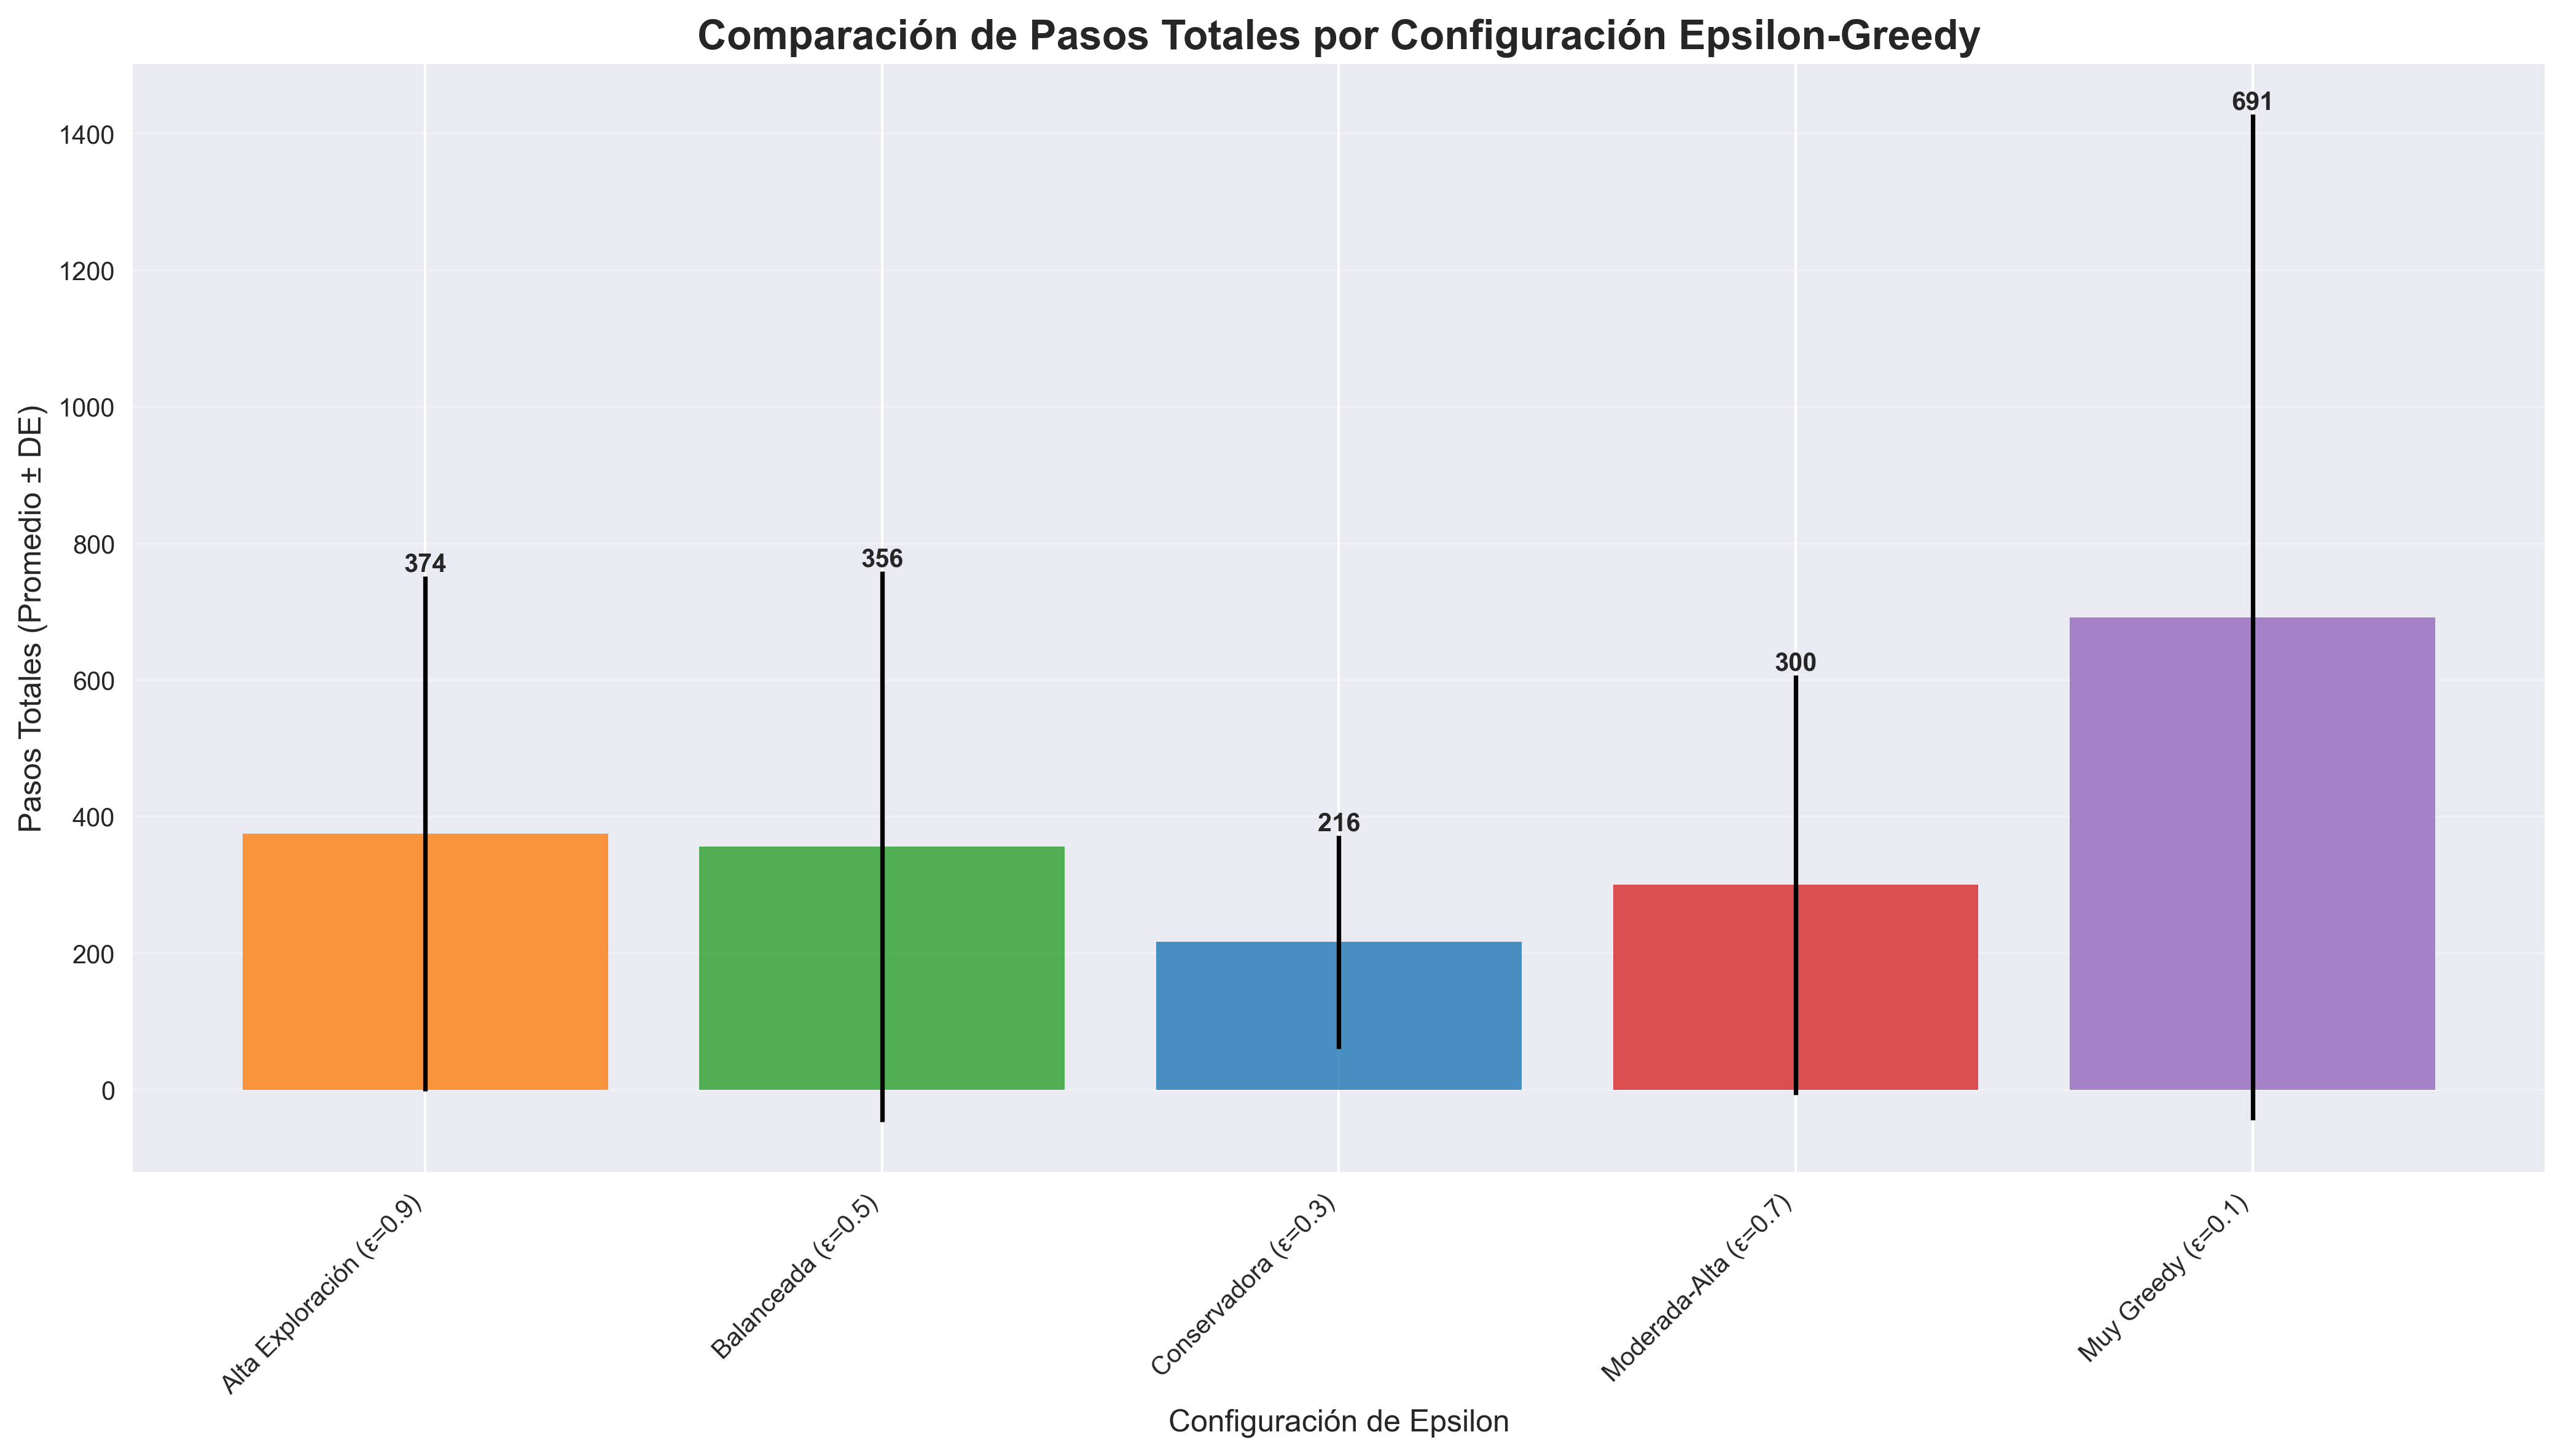
\includegraphics[width=1\textwidth]{epsilon_pasos_comparacion.png}
        \caption{Comparación de Pasos Totales.}
        \label{fig:epsilon_pasos}
\end{figure}
\begin{figure}[H]
        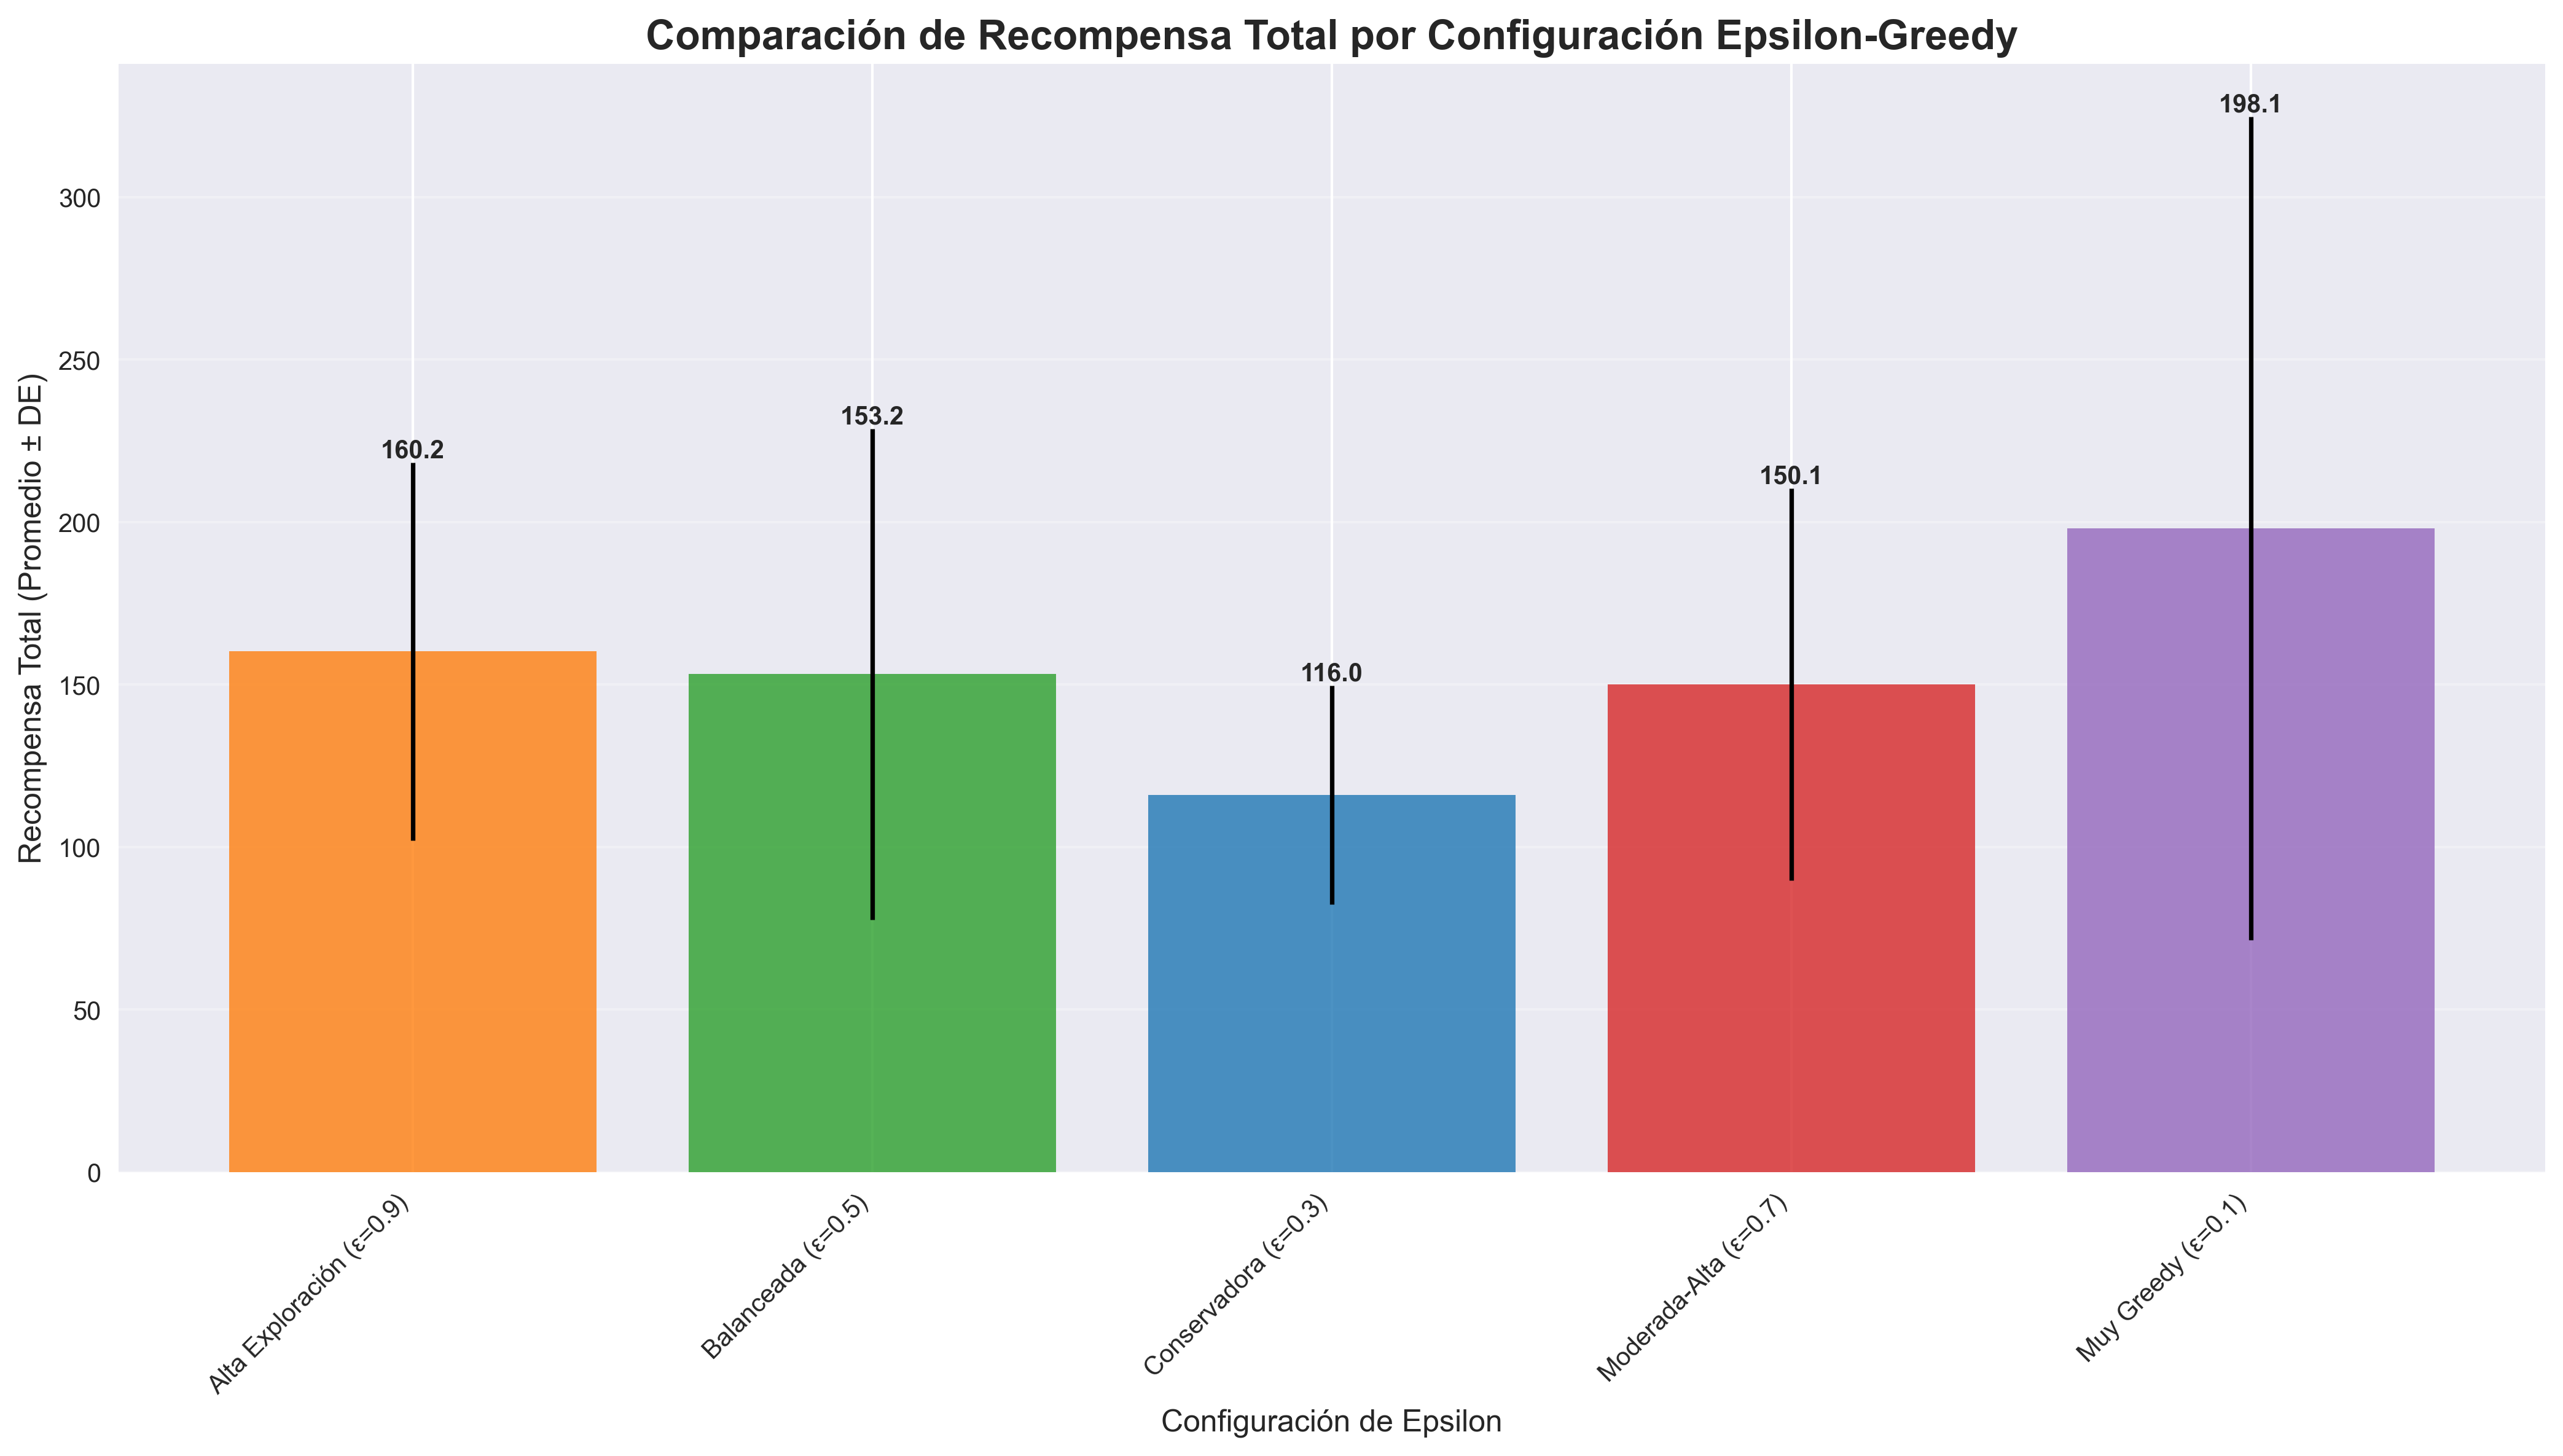
\includegraphics[width=1\textwidth]{epsilon_recompensa_comparacion.png}
        \caption{Comparación de Recompensa Total.}
        \label{fig:epsilon_recompensa}
\end{figure}

Como se observa en la Figura \ref{fig:epsilon_pasos} y \ref{fig:epsilon_recompensa}, la configuración con $\epsilon=0.3$ no solo minimizó los pasos, sino que también mantuvo una recompensa competitiva, indicando una trayectoria de alta calidad. Todas las configuraciones lograron una tasa de éxito del 100\%, lo que demuestra que, aunque ineficiente en algunos casos, Epsilon-Greedy es un método robusto para este problema.

\subsection{Análisis de los Algoritmos de Búsqueda}
Los algoritmos de búsqueda, al tener un modelo del mundo (el mapa), mostraron un rendimiento drásticamente superior en eficiencia.

% Se ajusta la tabla para que no exceda los márgenes de la página
\begin{table}[H]
\centering
\caption{Comparación de Algoritmos de Búsqueda}
\label{tab:search_comparison}
\resizebox{\textwidth}{!}{%
\begin{tabular}{|l|c|c|c|c|c|}
\hline
\textbf{Algoritmo} & \textbf{Pasos} &  \textbf{Recompensa} & \textbf{Éxito (\%)} & \textbf{Eficiencia (Rec/Paso)} \\
\hline
Breadth-First Search & 29 ± 16  & 19.1 ± 6.4 & 100.0 & 0.7400 ± 0.1800 \\
\hline
Hill Climbing (First Imp.) & 2 ± nan & 11.5 ± nan & 100.0 & 5.7600 ± nan \\
\hline
Hill Climbing (Random Restart) & 3 ± 1 & 11.9 ± 0.6 & 100.0 & 4.9800 ± 1.8200 \\
\hline
Hill Climbing (Steepest) & 3 ± 1 & 11.6 ± 0.1 & 100.0 & 4.3300 ± 2.0300 \\
\hline
Simulated Annealing & 14 ± 15 & 15.0 ± 4.8 & 100.0 & 2.9500 ± 3.3800 \\
\hline
\end{tabular}%
}
\end{table}

La Tabla \ref{tab:search_comparison} y la Figura \ref{fig:search_graphs} revelan varios hallazgos clave:
\begin{itemize}
    \item \textbf{Superioridad de Hill Climbing:} Todas las variantes de Hill Climbing resolvieron el problema en un número de pasos extremadamente bajo (2-3 en promedio). Esto se debe a que el problema de navegación en Pueblo Paleta es convexo: casi cualquier movimiento hacia la dirección general del laboratorio es un "buen" movimiento. Por lo tanto, un algoritmo "greedy" como Hill Climbing es excepcionalmente efectivo. La variante \textbf{First Improvement} fue la más rápida, al no necesitar evaluar todos los vecinos en cada paso.
    \item \textbf{Costo de BFS:} Breadth-First Search, aunque encontró una ruta óptima en términos de pasos (no la más corta, pero sí una muy buena), fue el menos eficiente. Su naturaleza de exploración exhaustiva lo hizo tomar un promedio de 29 pasos, significativamente más que los demás.
    \item \textbf{Rendimiento de Simulated Annealing:} Este algoritmo se situó en un punto intermedio. Su capacidad para tomar "malos" pasos le permitió explorar más que Hill Climbing, resultando en más pasos, pero aun así fue mucho más eficiente que BFS.
    \item \textbf{Tasa de Éxito y Eficiencia:} Todos los algoritmos probados (que produjeron resultados válidos) tuvieron una tasa de éxito del 100\%. Sin embargo, al observar la métrica de eficiencia (recompensa por paso), \textbf{Hill Climbing (First Improvement)} destaca como el claro ganador, obteniendo el máximo valor por cada acción realizada.
\end{itemize}

\begin{figure}[H]
        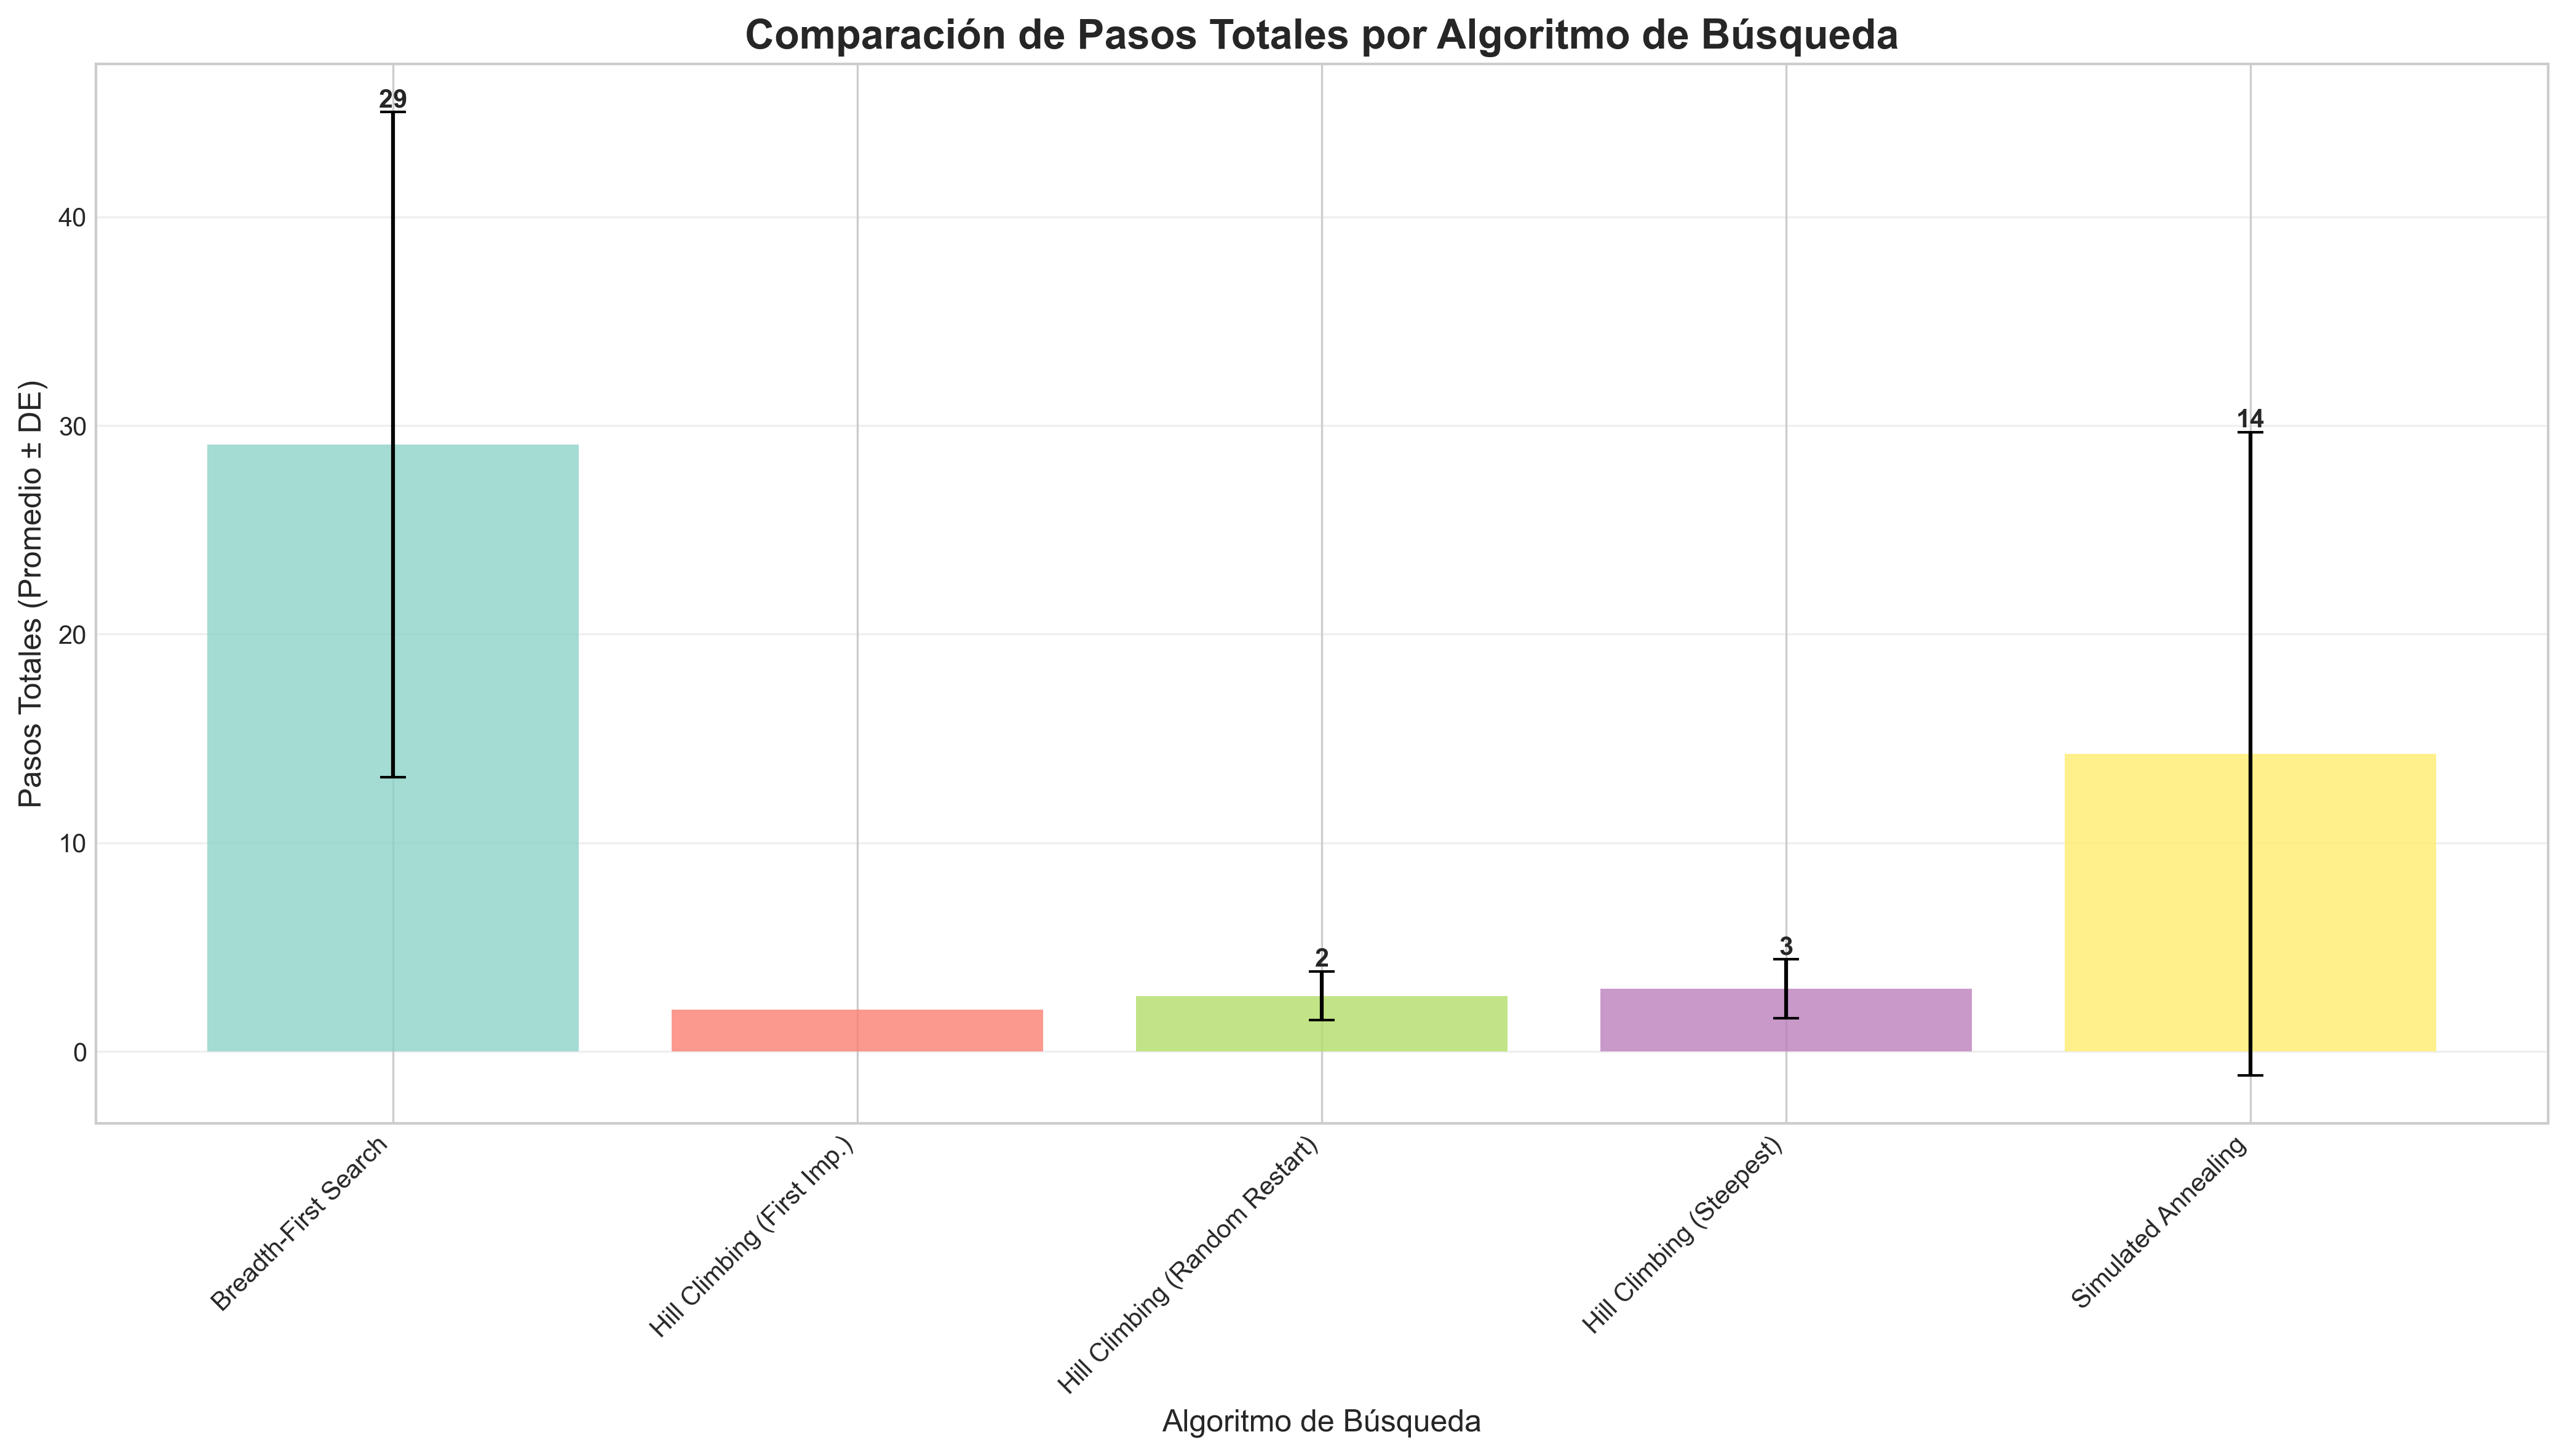
\includegraphics[width=1\textwidth]{search_pasos_comparacion.png}
        \caption{Comparación de Pasos Totales.}
        \label{fig:search_pasos}
\end{figure}
\begin{figure}[H]
        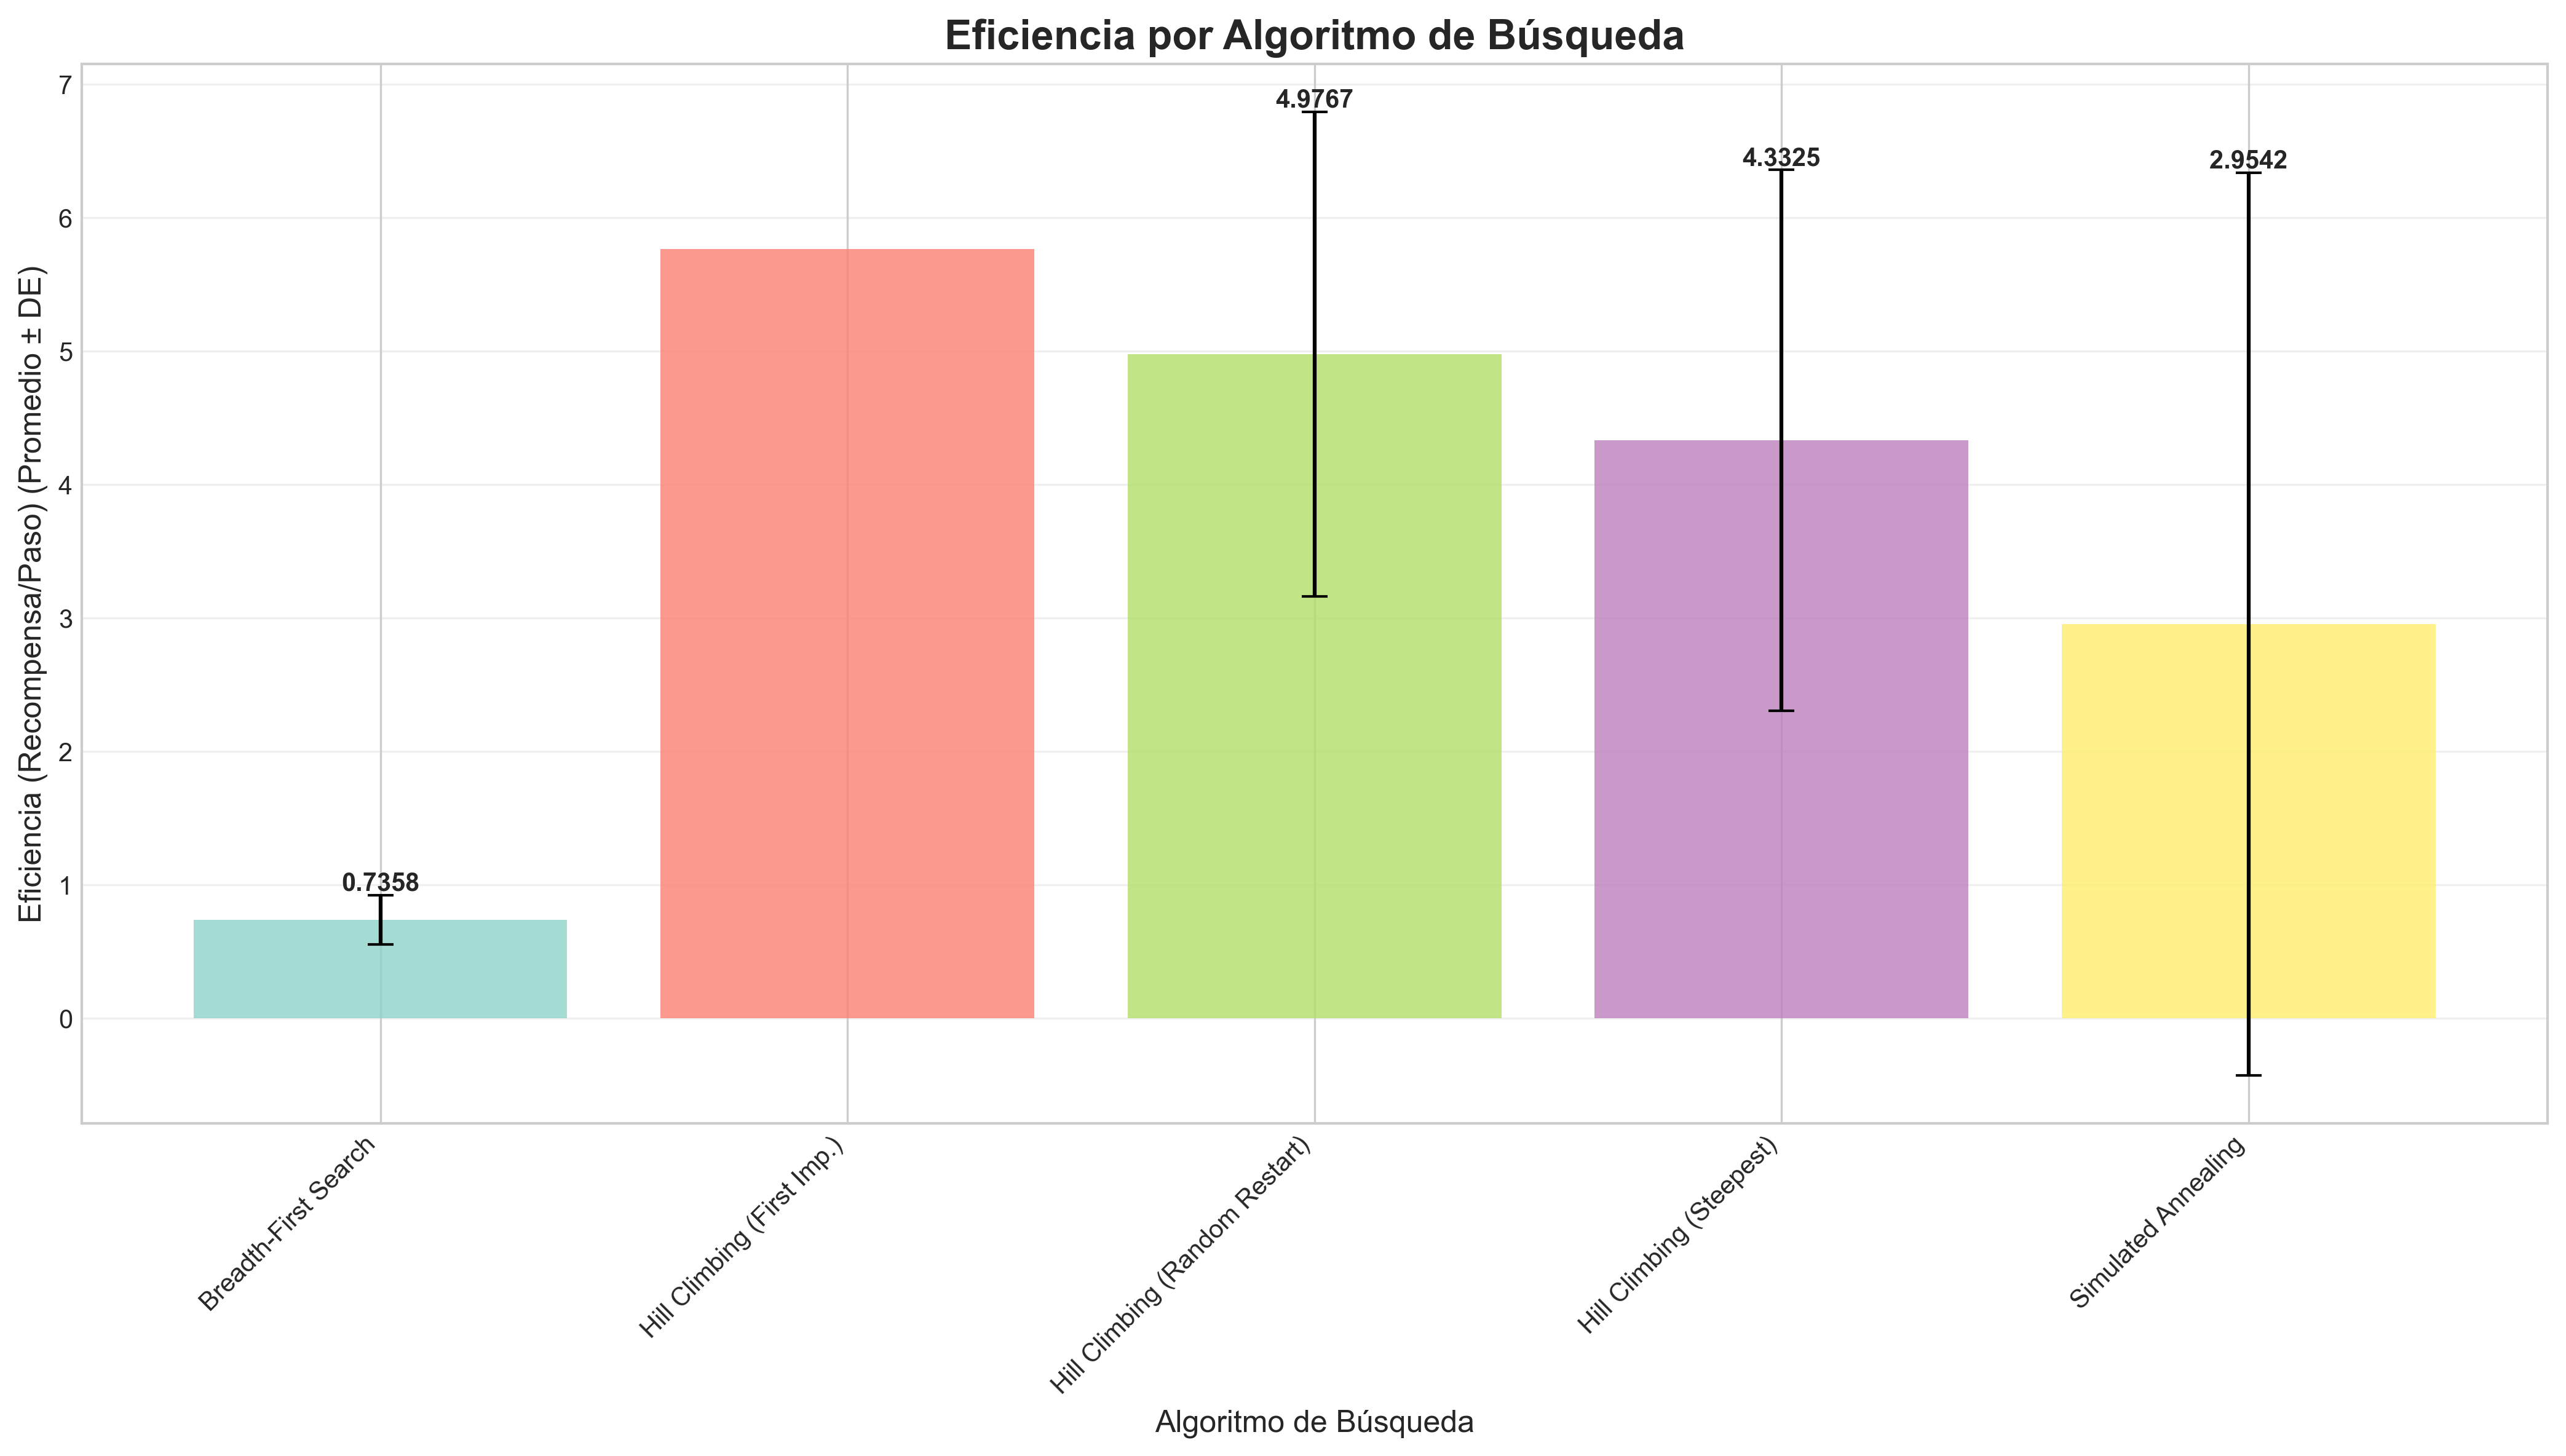
\includegraphics[width=1\textwidth]{search_eficiencia_comparacion.png}
        \caption{Comparación de Eficiencia (Recompensa/Paso).}
        \label{fig:search_eficiencia}
\end{figure}

Los algoritmos A* y Tabú Search no produjeron suficientes resultados válidos en las ejecuciones para ser incluidos en el análisis comparativo final, probablemente debido a timeouts o errores de implementación que los hicieron inviables en la práctica bajo las condiciones del experimento.

\subsection{Comparativa General: PPO vs. Epsilon-Greedy vs. Búsqueda}
Al comparar las tres familias de algoritmos, emerge una clara jerarquía de rendimiento para esta tarea específica:
\begin{enumerate}
    \item \textbf{Algoritmos de Búsqueda (Hill Climbing):} Indiscutiblemente los más eficientes. Resolvieron el problema en un puñado de pasos y en una fracción de segundo. Su desventaja es que requieren un conocimiento explícito del mapa y la posición del objetivo.
    \item \textbf{PPO (Aprendizaje por Refuerzo Profundo):} El agente PPO, aunque mucho más lento que los de búsqueda, demostró una política de navegación coherente, completando la tarea en un promedio de ~350 pasos y ~23 segundos. Su fortaleza radica en que no necesita un modelo del mundo; aprende directamente de la experiencia (píxeles), lo que lo hace más generalizable a tareas donde el mapa no se conoce de antemano.
    \item \textbf{Epsilon-Greedy:} Fue la estrategia menos eficiente en términos de tiempo y pasos. Aunque robusta, su método de aprendizaje simple y su exploración (a menudo aleatoria) la hacen inadecuada para problemas que requieren una secuencia larga y precisa de acciones, como lo demuestran sus tiempos de ejecución, que fueron órdenes de magnitud mayores que los de PPO.
\end{enumerate}

\begin{figure}[H]
    \centering
    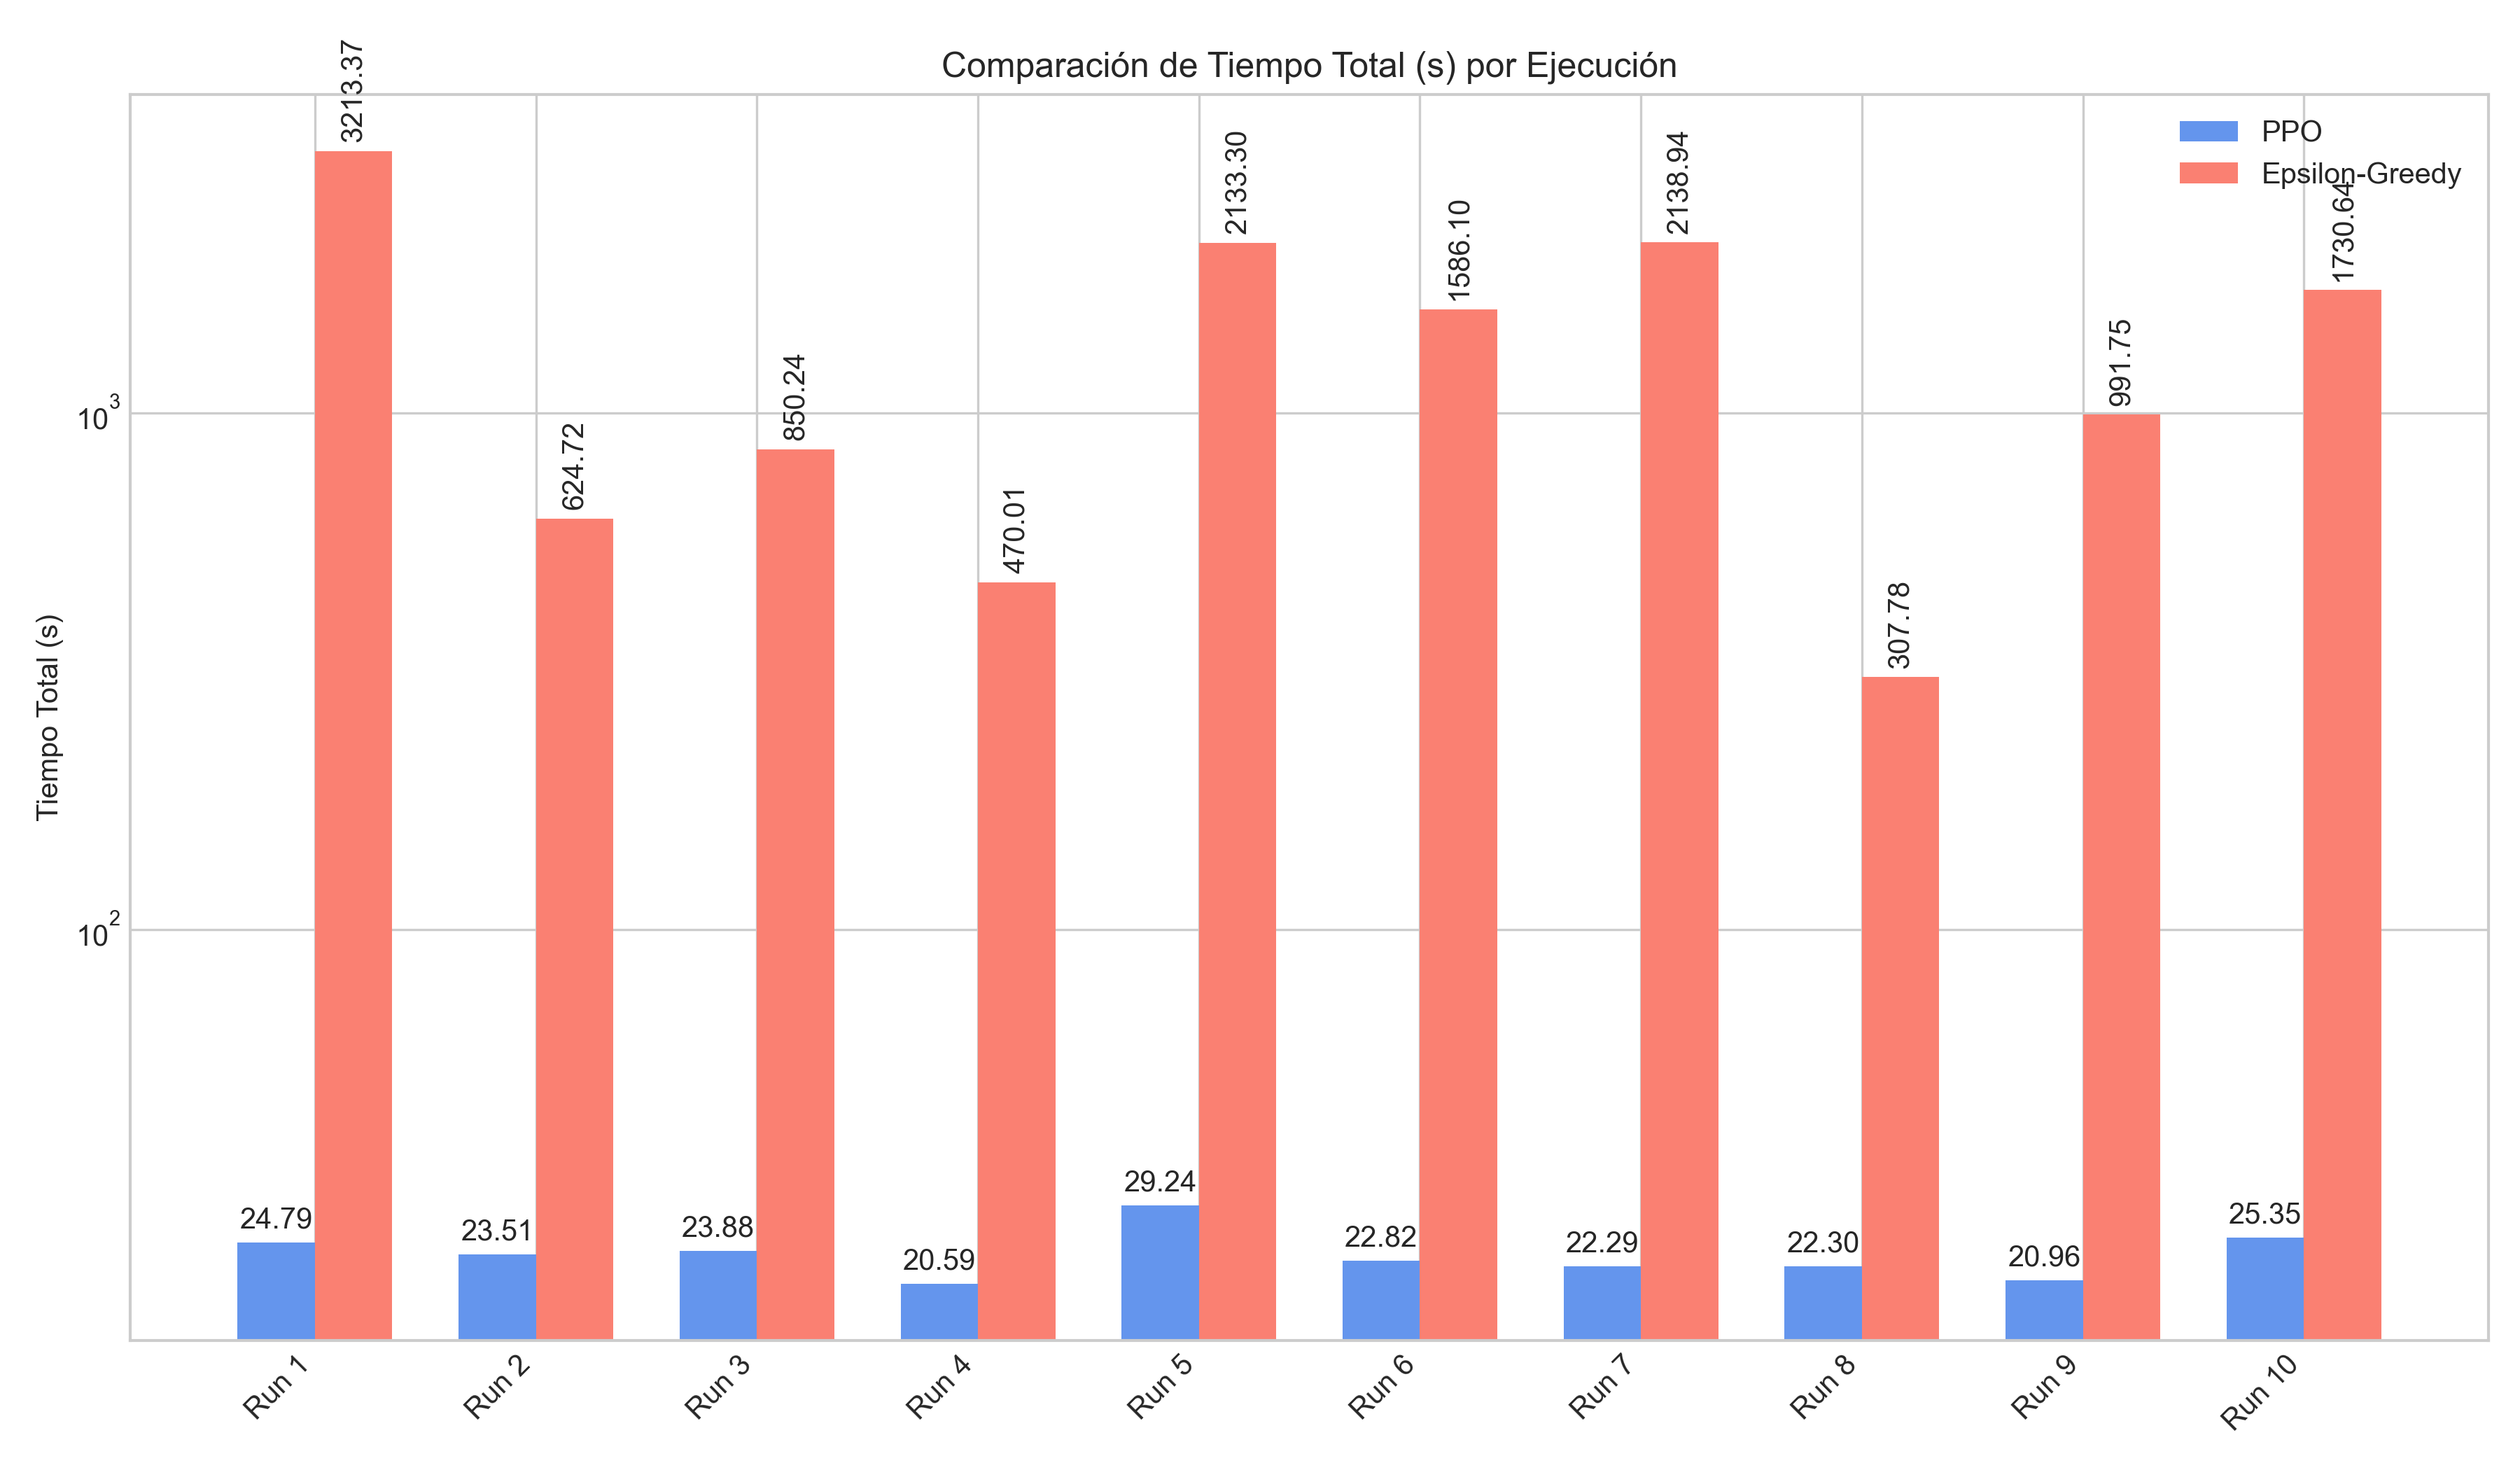
\includegraphics[width=1\textwidth]{tiempo_comparacion.png}
    \caption{Comparación de Tiempos de Ejecución Totales por tipo de Agente. Nótese la escala logarítmica en el eje Y, que evidencia la enorme diferencia de rendimiento.}
    \label{fig:tiempo_comparacion_general}
\end{figure}

La Figura \ref{fig:tiempo_comparacion_general} ilustra dramáticamente esta diferencia. Mientras que los algoritmos de búsqueda resuelven la tarea casi instantáneamente, PPO toma segundos y Epsilon-Greedy puede tardar minutos.

\section{Conclusiones}
\label{sec:conclusiones}

Este proyecto ha permitido realizar un análisis exhaustivo y comparativo de diferentes estrategias de inteligencia artificial aplicadas a un problema complejo y no estándar: la navegación inicial en \textit{Pokémon Rojo}. Los resultados obtenidos nos llevan a las siguientes conclusiones clave:

\begin{enumerate}
    \item \textbf{No existe una solución definitiva:} La elección del algoritmo óptimo depende críticamente de la naturaleza del problema y del conocimiento previo disponible. Para una tarea de navegación pura con un mapa conocido, los algoritmos de búsqueda clásicos como Hill Climbing son abrumadoramente superiores.
    \item \textbf{La eficiencia está en lo simple:} En entornos donde la función de recompensa es relativamente simple y monótona (como acercarse a un objetivo), los algoritmos "greedy" como Hill Climbing pueden superar a métodos más complejos. Su simplicidad computacional se traduce en una velocidad de decisión casi instantánea.
    \item \textbf{El Costo del Aprendizaje "End-to-End":} El agente PPO, que aprende directamente de los píxeles, es un enfoque mucho más general y potente. Sin embargo, esta generalidad tiene un costo computacional significativo, tanto en entrenamiento (no cubierto en este análisis) como en inferencia. Su rendimiento, aunque inferior al de los algoritmos de búsqueda, es notablemente bueno considerando que no tiene un modelo explícito del mundo.
    \item \textbf{Los Límites de Epsilon-Greedy:} La estrategia Epsilon-Greedy, aunque es un pilar en la teoría del aprendizaje por refuerzo, demuestra ser insuficiente para problemas con secuencias de acción largas y recompensas escasas. Su dependencia de la exploración aleatoria y una memoria simple de acciones pasadas la convierte en la estrategia menos eficiente de las analizadas.
    \item \textbf{La Importancia del Equilibrio Exploración-Explotación:} El análisis de las variantes de Epsilon-Greedy confirmó empíricamente la teoría. Tanto un exceso de exploración ($\epsilon=0.9$) como un exceso de explotación ($\epsilon=0.1$) conducen a un rendimiento deficiente. Un valor balanceado (en este caso, $\epsilon=0.3$) es crucial para encontrar soluciones eficientes.
    \item \textbf{El Entorno como Desafío Principal:} \textit{Pokémon Rojo} es un entorno de prueba formidable para la IA. Su alta dimensionalidad, recompensas escasas y naturaleza parcialmente observable lo convierten en un campo de pruebas ideal para algoritmos que buscan ir más allá de los benchmarks tradicionales.
    \item \textbf{Robustez vs. Eficiencia:} Mientras que los algoritmos de búsqueda fueron los más eficientes, su implementación puede ser frágil (como se vio con A* y Tabu Search, que fallaron en producir resultados consistentes). Estrategias como PPO y Epsilon-Greedy, aunque más lentas, demostraron ser más robustas y capaces de completar la tarea en el 100\% de los casos.
    \item \textbf{Ingeniería de Recompensas es Clave:} El éxito de cualquier agente de RL en este entorno está fuertemente ligado al diseño de la función de recompensa. Una buena función de recompensa puede guiar a un agente simple hacia el éxito, mientras que una mala puede hacer que incluso el algoritmo más avanzado falle.
    \item \textbf{El Valor de la Simulación de Alta Velocidad:} Los experimentos con los algoritmos de búsqueda se beneficiaron enormemente de un runner simplificado que se ejecutaba a máxima velocidad. Esto demuestra el potencial de desacoplar la lógica del agente de la renderización del emulador para acelerar la investigación y la experimentación.
\end{enumerate}

\noindent Para finalizar, este trabajo no solo ha identificado las estrategias más efectivas para un objetivo concreto, sino que también ha proporcionado una profunda visión sobre las fortalezas, debilidades y compromisos inherentes a cada familia de algoritmos de inteligencia artificial cuando se enfrentan a un desafío del mundo real, amplio y, sobre todo, complejo.
\end{document}
